\documentclass[pdftex,12pt,xcolor=svgnames]{beamer}

\mode<presentation>
{
  \usetheme{boxes}
  \usecolortheme[named=MidnightBlue]{structure}
  %\setbeamercolor{normal text}{bg=NavajoWhite!20}
  \usefonttheme{serif}
  \setbeamertemplate{navigation symbols}{}
  % Show frame number and author name in footline
  \setbeamertemplate{footline}[frame number]
  \addtobeamertemplate{footline}{\quad\textcolor{gray}{James Robert Lloyd}}{}
  % Set frame titles in small capitals
  \setbeamerfont{frametitle}{shape=\scshape,family=\rmfamily}
  \setbeamercolor{frametitle}{bg=gray!60!white,fg=black}
  % Alerted text: blue (uncomment second line if theme sets alerted text to bold)
  \setbeamercolor{alerted text}{fg=blue}
  %\setbeamerfont*{alerted text}{}
  \setbeamertemplate{bibliography item}[text] %{\hbox{\donotcoloroutermaths$\blacktriangleright$}}
  \setbeamertemplate{bibliography entry title}{}
  \setbeamertemplate{bibliography entry author}{}
  \setbeamertemplate{bibliography entry note}{}
  \setbeamertemplate{bibliography entry location}{}

}
\usepackage[english]{babel}
\usepackage[latin1]{inputenc}
\usepackage{times}
\usepackage[T1]{fontenc}
\usepackage{hyperref}
\usepackage{multimedia}
\usepackage{eepic}
\usepackage{graphicx}
%\usepackage[nohug]{latexinclude/diagrams}
\usepackage{tikz}
\usetikzlibrary{calc}

%% \newcommand{\footlineextra}[1]{
%%     \begin{tikzpicture}[remember picture,overlay]
%%         \node[yshift=1.5ex,anchor=south east] at (current page.south east)
%% {#1};
%%     \end{tikzpicture}
%% }

\newcommand{\footlineextra}[1]{
    \begin{tikzpicture}[remember picture,overlay]
        \node[xshift=-5ex,yshift=-0.5ex,anchor=south east] at (current page.south east)
             {\mbox{\tiny \textcolor{MidnightBlue}{#1}}};
    \end{tikzpicture}
}

\def\sectionframe#1{
  {
    \setbeamertemplate{footline}{\empty}
    \begin{frame}{}
      \begin{center}
        \huge\sc #1
      \end{center}
    \end{frame}
  }
}


\usepackage{etex}
%% This file provides examples of some useful macros for typesetting
% dissertations.  None of the macros defined here are necessary beyond
% for the template documentation, so feel free to change, remove, and add
% your own definitions.
%
% We recommend that you define macros to separate the semantics
% of the things you write from how they are presented.  For example,
% you'll see definitions below for a macro \file{}: by using
% \file{} consistently in the text, we can change how filenames
% are typeset simply by changing the definition of \file{} in
% this file.
% 
%% The following is a directive for TeXShop to indicate the main file
%%!TEX root = diss.tex

\newcommand{\pd}{\mbox{pd}}
\newcommand{\tr}{\mbox{tr}}
\newcommand{\mbf}[1]{\mbox{\boldmath $#1$}}
\newcommand{\deriv}[2]{\frac{\partial #1}{\partial #2}}
\newcommand{\mean}{\mathop{\mbox{mean}}}
\newcommand{\median}{\mathop{\mbox{median}}}
\newcommand{\diag}{\mbox{diag}}
\newcommand{\trace}{\mbox{trace}}
\newcommand{\st}{\mbox{st}}
\newcommand{\FF}{\tilde{F}}
\newcommand{\cut}[1]{}
\newcommand{\vn}{\varnothing}
\def\argmax{\operatornamewithlimits{arg\,max}}
\def\argmin{\operatornamewithlimits{arg\,min}}
\def\theequation{\arabic{section}.\arabic{equation}}
\def\thedefinition{\arabic{section}.\arabic{definition}}
\def\thetheorem{\arabic{section}.\arabic{theorem}}
\def\theexample{\arabic{section}.\arabic{example}}

\newcommand{\NA}{\textsc{n/a}}	% for "not applicable"
\newcommand{\eg}{e.g.,\ }	% proper form of examples (\eg a, b, c)
\newcommand{\ie}{i.e.,\ }	% proper form for that is (\ie a, b, c)
\newcommand{\etal}{\emph{et al}}

\newcommand{\expect}{\mathbb{E}}
\newcommand{\variance}{\mathbb{V}}
\newcommand{\bx}{{\bf x}}
\newcommand{\by}{{\bf y}}
\newcommand{\bX}{{\bf X}}
\newcommand{\bK}{{\bf K}}
\newcommand{\bs}{{\bf s}}
\newcommand{\bu}{{\bf u}}
\newcommand{\bff}{{\bf f}}

%\documentclass[usenames,dvipsnames]{beamer}
%\usepackage{beamerthemesplit}
%\usepackage{graphics}
%\usepackage{amsmath}
%\usepackage{rotating}
%\usepackage{array}
%\usepackage{nth}
\usepackage{xcolor}
\usepackage{textcomp}
\usepackage{listings}
%\usepackage[usenames,dvipsnames]{color}
% This is the color used for MATLAB comments below
\definecolor{MatlabDarkGreen}{rgb}{0.0,0.4,0.0}
\definecolor{Blue}{rgb}{0.0,0.0,1.0}

% For faster processing, load Matlab syntax for listings
\lstloadlanguages{Matlab}%
\lstset{language=Matlab,                        % Use MATLAB
        frame=single,                           % Single frame around code
        basicstyle=\tiny\ttfamily,             % Use small true type font
        keywordstyle=[1]\color{Blue}\bf,        % MATLAB functions bold and blue
        keywordstyle=[2]\color{Purple},         % MATLAB function arguments purple
        keywordstyle=[3]\color{Blue}\underbar,  % User functions underlined and blue
        identifierstyle=,                       % Nothing special about identifiers
                                                % Comments small dark green courier
        commentstyle=\usefont{T1}{pcr}{m}{sl}\color{MatlabDarkGreen}\tiny,
        stringstyle=\color{Purple},             % Strings are purple
        showstringspaces=false,                 % Don't put marks in string spaces
        tabsize=5,                              % 5 spaces per tab
        %
        %%% Put standard MATLAB functions not included in the default
        %%% language here
        morekeywords={xlim,ylim,var,alpha,factorial,poissrnd,normpdf,normcdf},
        %
        %%% Put MATLAB function parameters here
        morekeywords=[2]{on, off, interp},
        %
        %%% Put user defined functions here
        morekeywords=[3]{FindESS, homework_example},
        %
        morecomment=[l][\color{Blue}]{...},     % Line continuation (...) like blue comment
        numbers=left,                           % Line numbers on left
        firstnumber=1,                          % Line numbers start with line 1
        numberstyle=\tiny\color{Blue},          % Line numbers are blue
        stepnumber=50                            % Line numbers go in steps of 5
        }

% Includes a MATLAB script.
% The first parameter is the label, which also is the name of the script
%   without the .m.
% The second parameter is the optional caption.
\newcommand{\matlabscript}[2]
  {\begin{itemize}\item[]\lstinputlisting[caption=#2,label=#1]{#1.m}\end{itemize}}


\usepackage{tabularx}
\usepackage{picins}
\usepackage{tikz}
\usepackage{changepage}

\usetikzlibrary{shapes.geometric,arrows,chains,matrix,positioning,scopes,calc}
\tikzstyle{mybox} = [draw=white, rectangle]

\definecolor{camlightblue}{rgb}{0.601 , 0.8, 1}
\definecolor{camdarkblue}{rgb}{0, 0.203, 0.402}
\definecolor{camred}{rgb}{1, 0.203, 0}
\definecolor{camyellow}{rgb}{1, 0.8, 0}
\definecolor{lightblue}{rgb}{0, 0, 0.80}
\definecolor{white}{rgb}{1, 1, 1}
\definecolor{whiteblue}{rgb}{0.80, 0.80, 1}

\newcolumntype{x}[1]{>{\centering\arraybackslash\hspace{0pt}}m{#1}}
\newcommand{\tabbox}[1]{#1}

%%%%%%%%%%%%%%%%%%%%%%%%%%%%%%%%%%%%%%%%%%%
%
% Some look and feel definitions
%
%%%%%%%%%%%%%%%%%%%%%%%%%%%%%%%%%%%%%%%%%%%

\setlength{\columnsep}{0.03\textwidth}
\setlength{\columnseprule}{0.0018\textwidth}
\setlength{\parindent}{0.0cm}

%% This file provides examples of some useful macros for typesetting
% dissertations.  None of the macros defined here are necessary beyond
% for the template documentation, so feel free to change, remove, and add
% your own definitions.
%
% We recommend that you define macros to separate the semantics
% of the things you write from how they are presented.  For example,
% you'll see definitions below for a macro \file{}: by using
% \file{} consistently in the text, we can change how filenames
% are typeset simply by changing the definition of \file{} in
% this file.
% 
%% The following is a directive for TeXShop to indicate the main file
%%!TEX root = diss.tex

\newcommand{\pd}{\mbox{pd}}
\newcommand{\tr}{\mbox{tr}}
\newcommand{\mbf}[1]{\mbox{\boldmath $#1$}}
\newcommand{\deriv}[2]{\frac{\partial #1}{\partial #2}}
\newcommand{\mean}{\mathop{\mbox{mean}}}
\newcommand{\median}{\mathop{\mbox{median}}}
\newcommand{\diag}{\mbox{diag}}
\newcommand{\trace}{\mbox{trace}}
\newcommand{\st}{\mbox{st}}
\newcommand{\FF}{\tilde{F}}
\newcommand{\cut}[1]{}
\newcommand{\vn}{\varnothing}
\def\argmax{\operatornamewithlimits{arg\,max}}
\def\argmin{\operatornamewithlimits{arg\,min}}
\def\theequation{\arabic{section}.\arabic{equation}}
\def\thedefinition{\arabic{section}.\arabic{definition}}
\def\thetheorem{\arabic{section}.\arabic{theorem}}
\def\theexample{\arabic{section}.\arabic{example}}

\newcommand{\NA}{\textsc{n/a}}	% for "not applicable"
\newcommand{\eg}{e.g.,\ }	% proper form of examples (\eg a, b, c)
\newcommand{\ie}{i.e.,\ }	% proper form for that is (\ie a, b, c)
\newcommand{\etal}{\emph{et al}}

\newcommand{\expect}{\mathbb{E}}
\newcommand{\variance}{\mathbb{V}}
\newcommand{\bx}{{\bf x}}
\newcommand{\by}{{\bf y}}
\newcommand{\bX}{{\bf X}}
\newcommand{\bK}{{\bf K}}
\newcommand{\bs}{{\bf s}}
\newcommand{\bu}{{\bf u}}
\newcommand{\bff}{{\bf f}}

\usepackage{preamble}
\hypersetup{colorlinks=true,citecolor=blue}
%\pdfmapfile{+sansmathaccent.map}

\title{Automatic construction and description of nonparametric models}

\author{
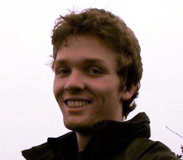
\includegraphics[height=0.2\textwidth]{figures/JamesLloyd4}
\qquad
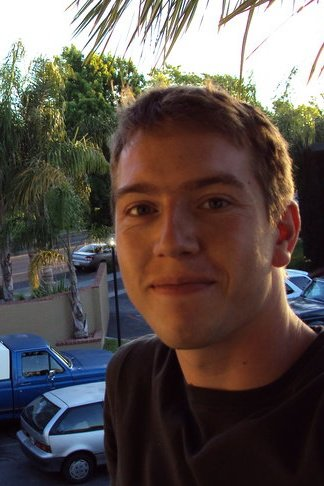
\includegraphics[height=0.2\textwidth, trim=20mm 25mm 0mm 25mm, clip]{figures/david2}
\qquad
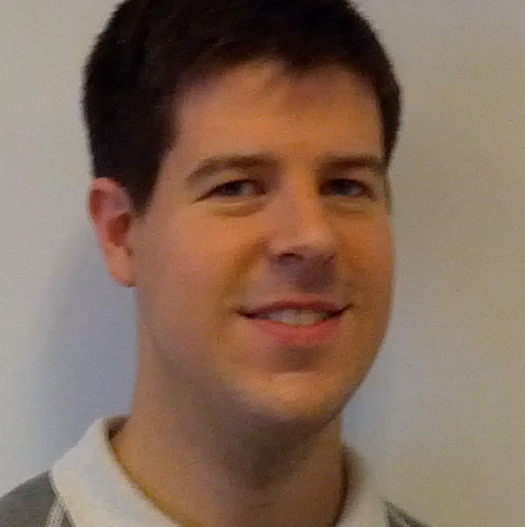
\includegraphics[height=0.2\textwidth]{figures/roger-photo}
\\
James Robert Lloyd, David Duvenaud, Roger Grosse,\\ Joshua B. Tenenbaum, Zoubin Ghahramani
}
\institute{
%\includegraphics[width=0.4\textwidth]{figures/spiral_main}
}
%\date{}


\begin{document}

\frame[plain] {
\titlepage
}

\setbeamercolor{toc}{fg=black}

%\frame[plain] {
%\frametitle{Outline}
%\tableofcontents

%\begin{itemize} 
%	\item Motivation
%	\item Automated structure discovery in regression
%	\begin{itemize} 
%		\item Gaussian process regression
%		\item Structures expressible through kernel composition
%		\item A massive missing piece
%		\item grammar \& search over models
%		\item Examples of structures discovered
%	\end{itemize}
%	\item Automated structure discovery in matrix models
%	\begin{itemize} 
%		\item expressing models as matrix decompositions
%		\item grammar \& special cases
%		\item examples of structures discovered on images
%	\end{itemize}
%\end{itemize}   
%
%}


%\frame[plain]{
%\frametitle{Credit where credit is due}
%
%Talk based on two papers:
%	\begin{itemize}
%		\item Structure Discovery in Nonparametric Regression through Compositional Kernel Search [ICML 2013]
%		\\
%		{David Duvenaud, James Robert Lloyd, Roger Grosse, Joshua B. Tenenbaum, Zoubin Ghahramani}
%		\item Exploiting compositionality to explore a large space of model structures [UAI 2012]
%		\\
%		Roger B. Grosse, Ruslan Salakhutdinov, \\William T. Freeman, Joshua B. Tenenbaum
%	\end{itemize}
%}


\frame[plain]{
\frametitle{Typical statistical modelling}
\begin{itemize} 
	\item Statistical / machine learning models typically built by hand, or chosen from a fixed set
	\begin{itemize} 
	  \vspace{\baselineskip}
		\item Example: Scikit-learn
	\end{itemize}
\end{itemize}
\begin{center}
		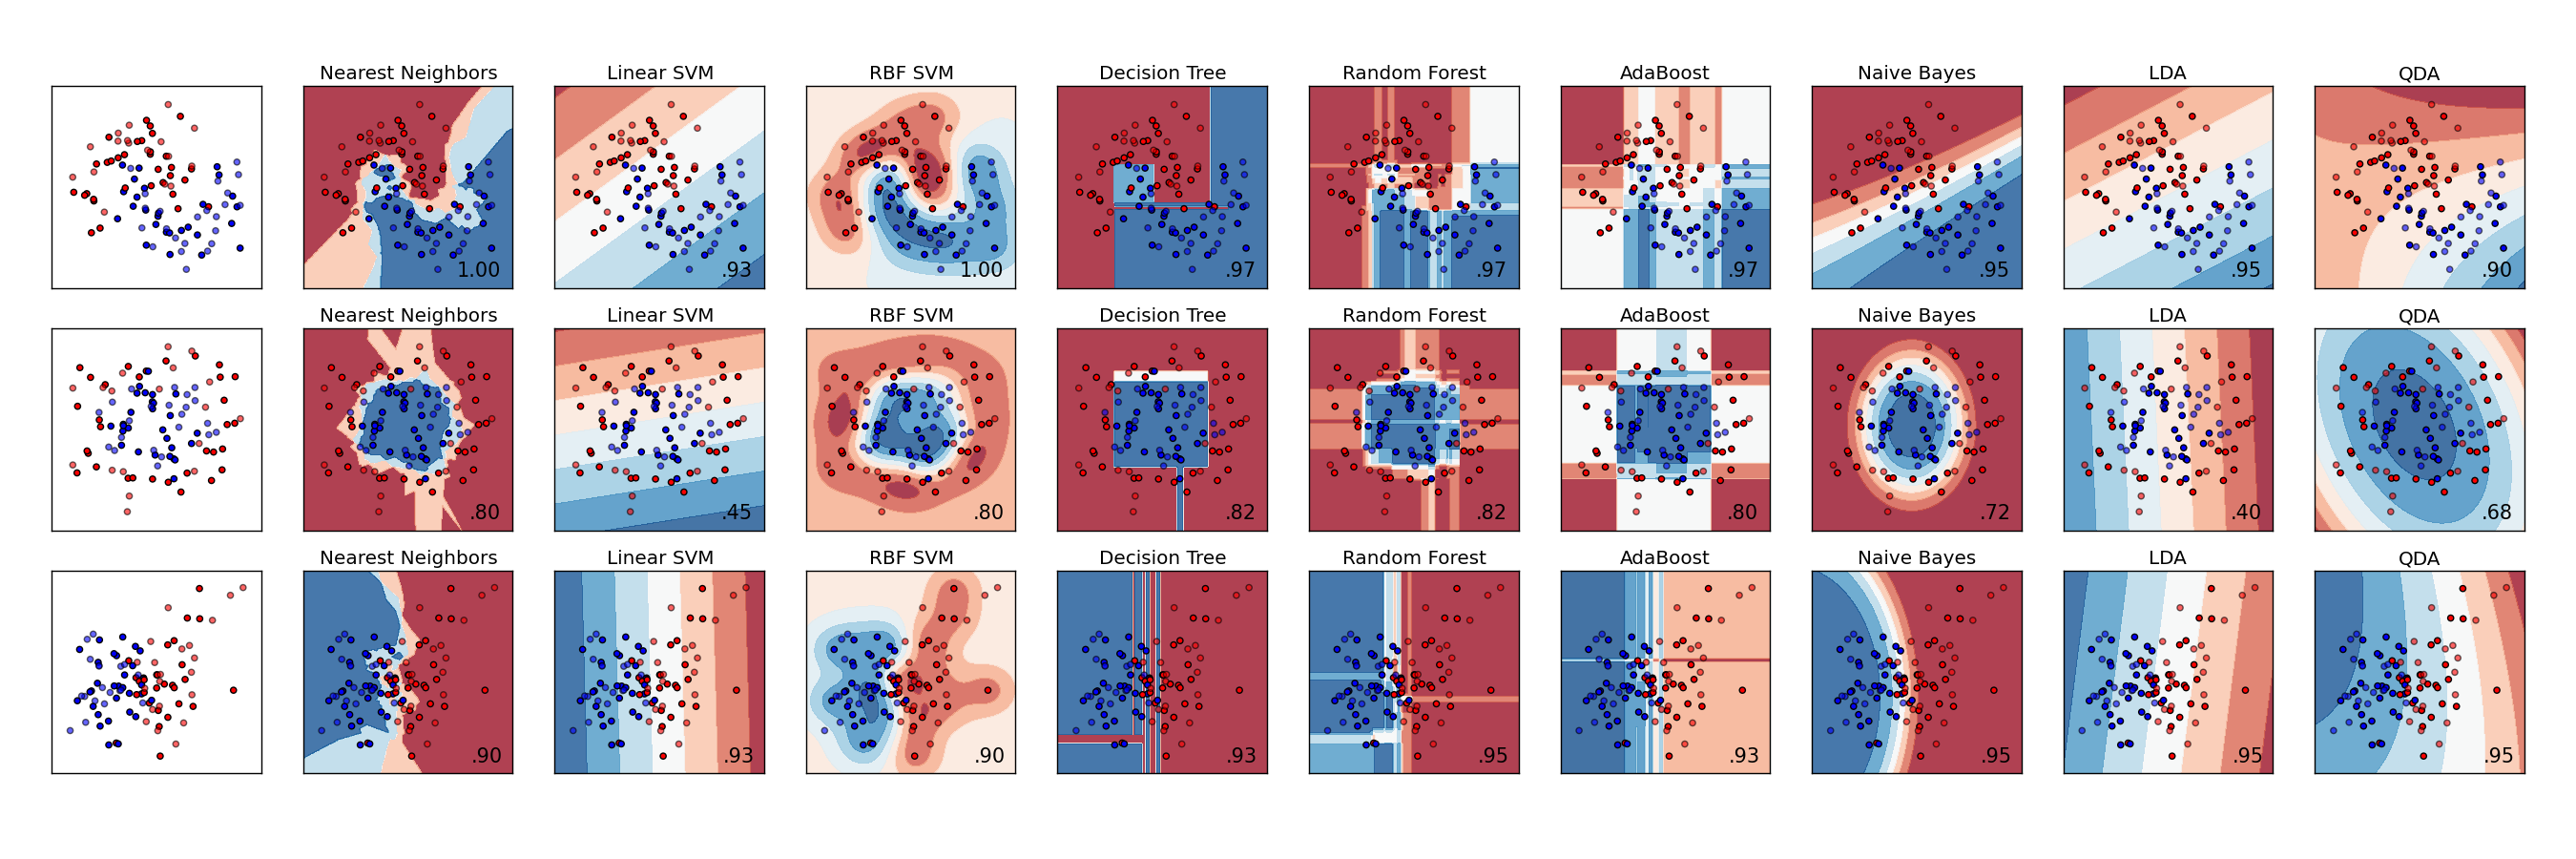
\includegraphics[width=9cm, trim=1.39cm 15cm 35cm 0cm, clip]{figures/plot_classifier_comparison_1}\\
		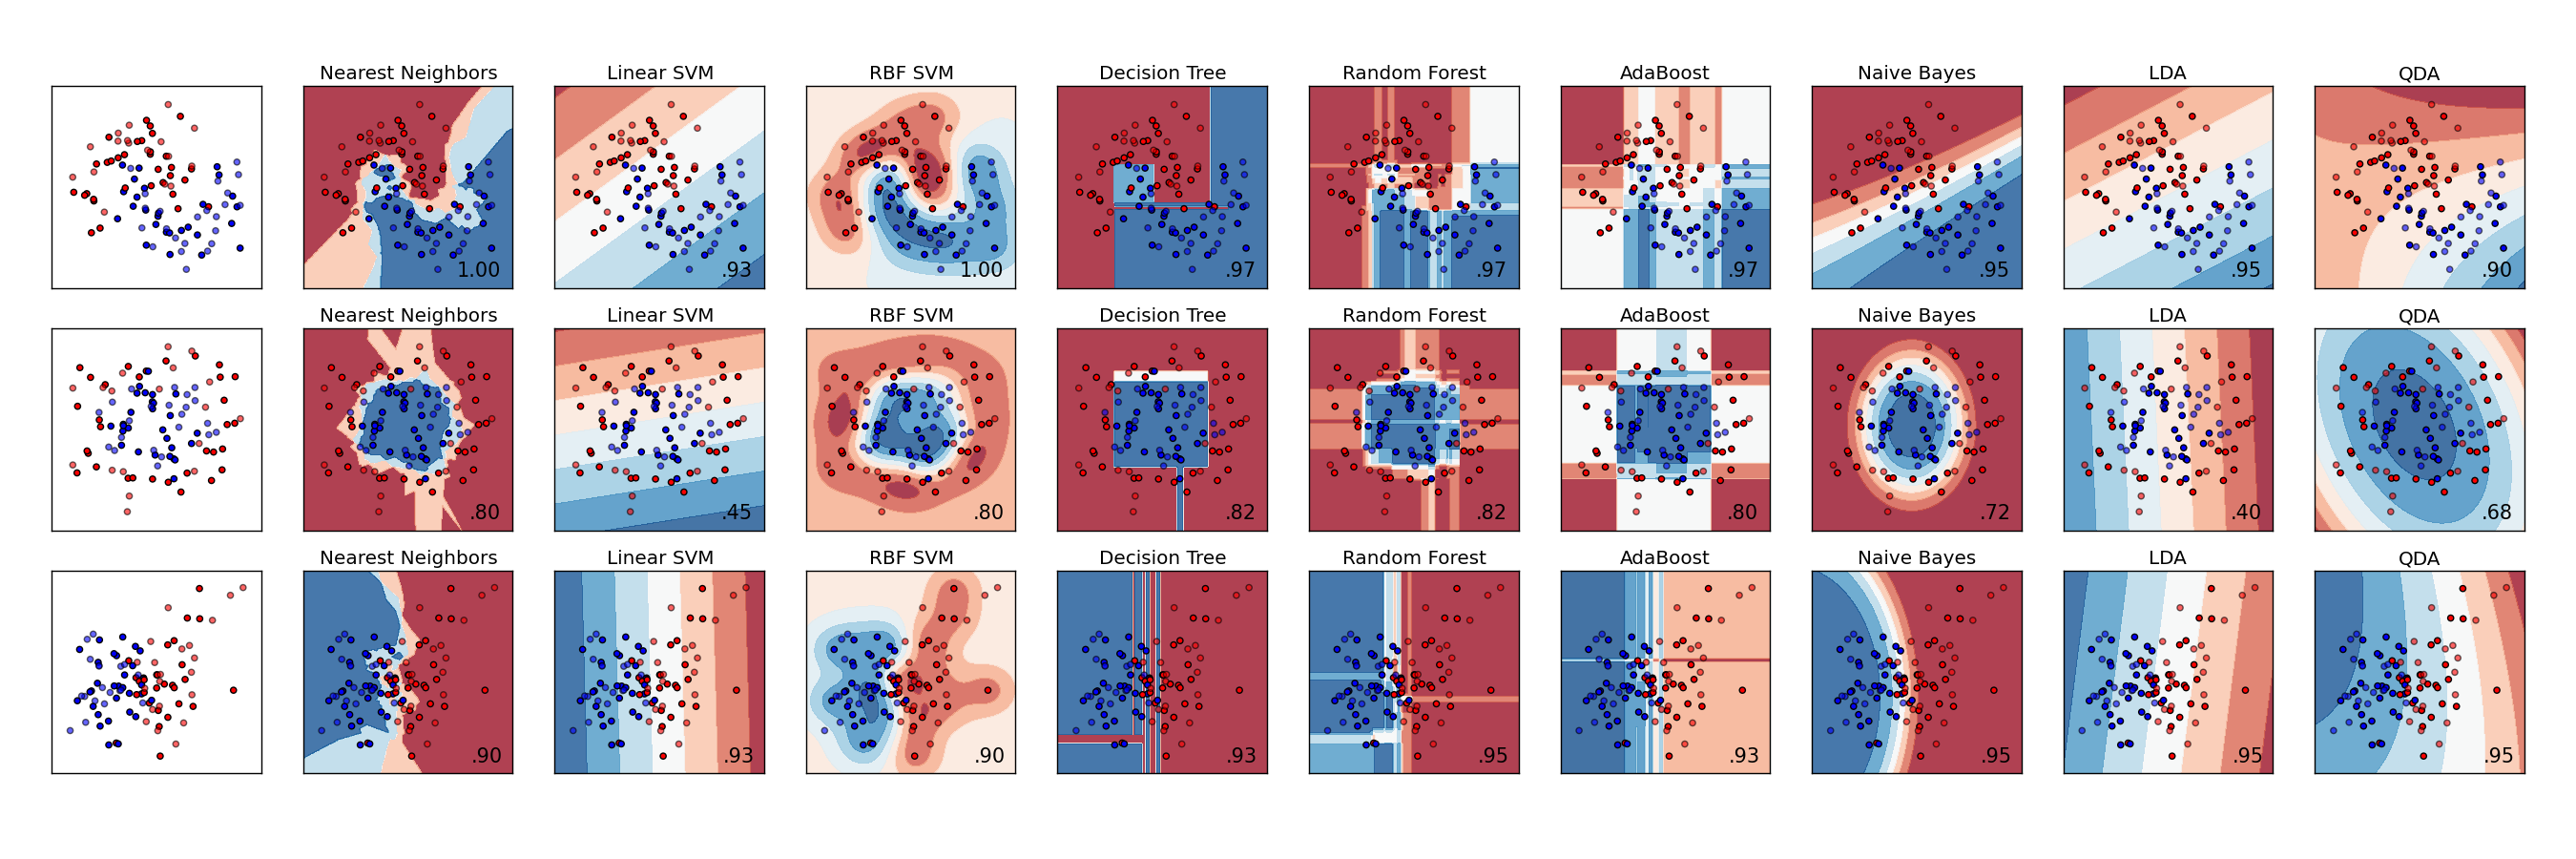
\includegraphics[width=9cm, trim=35cm 15cm 1.35cm 0cm, clip]{figures/plot_classifier_comparison_1}
\end{center}
}




\frame[plain]{
\frametitle{This approach is limited}
\begin{itemize} 
	\item Building by hand requires considerable expertise% and understanding of the dataset 
	\begin{itemize}
	  \item Can become an entire research project
	\end{itemize}
	\vspace{\baselineskip}
	\item Just being nonparametric isn't good enough
	\begin{itemize}
	  \item Nonparametric does not mean assumption free!
	\end{itemize}
	\vspace{\baselineskip}
	\item Can silently fail
	\begin{itemize}
	  \item If none of the models tried fit the data well, how can you tell?
	\end{itemize}
\end{itemize}
}



\frame[plain]{
\frametitle{Can we do better?}
	\begin{itemize} 
	\item Andrew Gelman asks:  How can an AI do statistics?
	\vspace{\baselineskip}
	\item An artificial statistician would need:
			\begin{itemize} 
			\item a language for describing arbitrarily complicated models
			\item a method of searching over those models
			\item a procedure to check model fit
		\end{itemize}
	\vspace{\baselineskip}
	\item We constructed such a language over regression models, a procedure to search over it, and a method to describe in natural language the properties of the resulting models
	\begin{itemize}
		\item Actively researching automatic model-checking\ldots
	\end{itemize}
\end{itemize}
}


\definecolor{verylightblue}{rgb}{0.97,0.97,1}
\setlength{\fboxsep}{0pt}

\newcommand{\ltrim}{ 2 }
\newcommand{\rictrim}{ 2 }
%\newcommand{\airlinefig}[1]{\includegraphics[trim=20 0 12 20, clip, width=0.207\textwidth]{figures/#1}}
%\newcommand{\airlinefigtwo}[1]{}
\newcommand{\olduptext}[1]{\hspace{-1cm} \raisebox{ 0.8cm}{ {#1}} \hspace{-0.75cm} }
\newcommand{\uptext}[1]{\raisebox{1cm}{#1}}

\frame[plain]{
\frametitle{Example: An automatic analysis}


\begin{adjustwidth}{-1.2cm}{}
\begin{tabular}{@{}c@{}}
%\airlinefig{01-airline-months_all}&\hspace{0.6cm}\olduptext{$=$} \hspace{-0.1cm}
%\airlinefig{01-airline-months_1} & \olduptext{$+$}
%\airlinefig{01-airline-months_2} & \olduptext{$+$}
%\airlinefig{/01-airline-months_3} \\
%\hspace{-3.5mm}
%\fbox{

%\hspace{-3.5mm}
\begin{tabular}{@{}cc@{}}
%\\[-0.7em]
%\fcolorbox{blue}{white}{
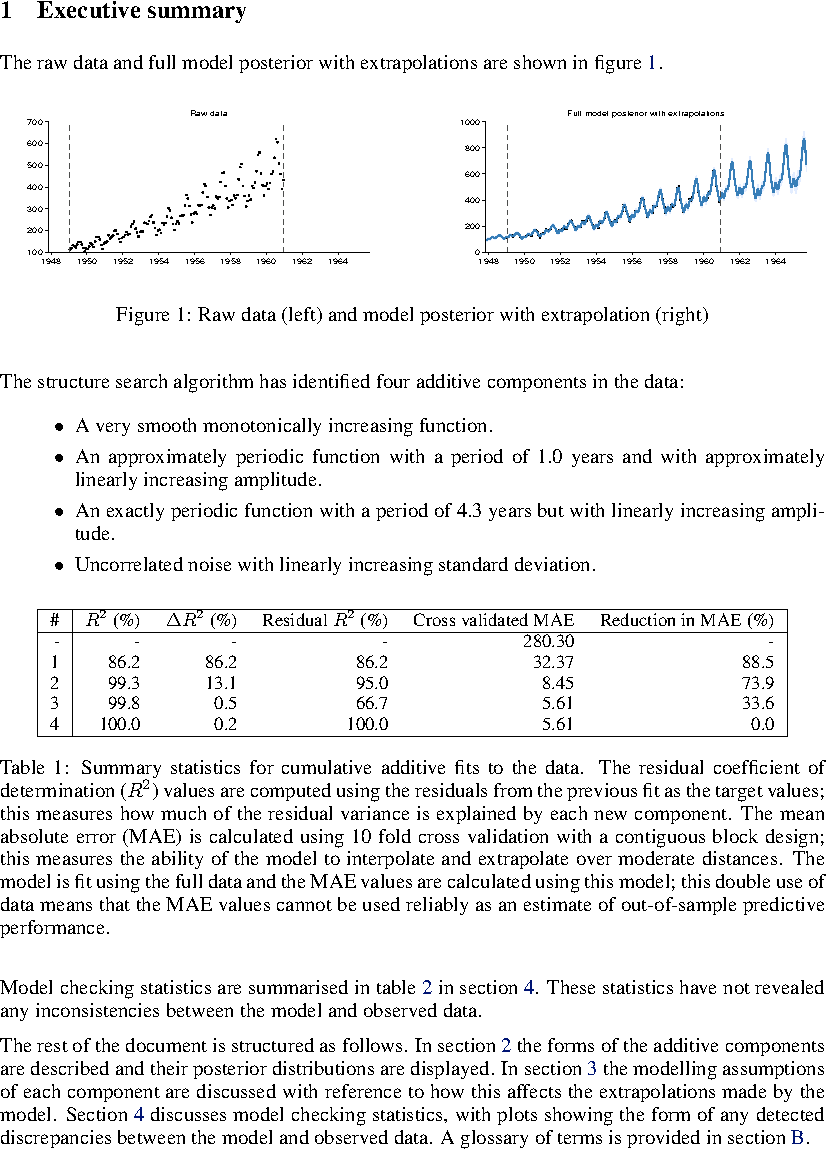
\includegraphics[trim=7.8cm 14.5cm 0cm 2cm, clip, width=0.5\columnwidth]{figures/airline-pages/pg_0002-crop} 
%}
 & \uptext{$=$} \\
%{\scriptsize Original data} & 
\end{tabular}

\\
\begin{tabular}{p{3.45cm}p{0.3cm}p{3.45cm}p{0.3cm}p{3.45cm}}
\\%[1cm]
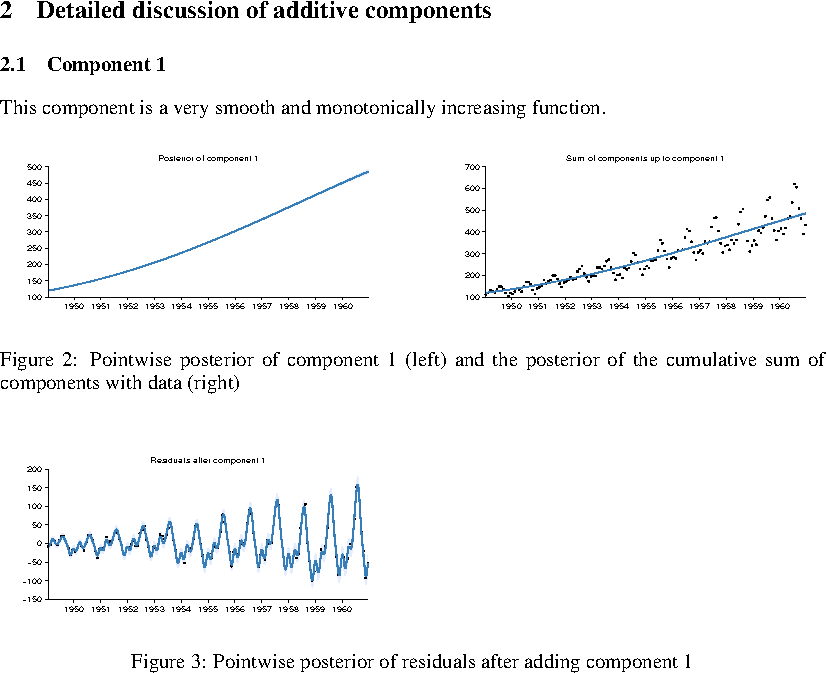
\includegraphics[trim=0.4cm 6cm 8.4cm 2.75cm, clip, width=0.33\columnwidth]{figures/airline-pages/pg_0003-crop} & 
 \uptext{$+$}  &  
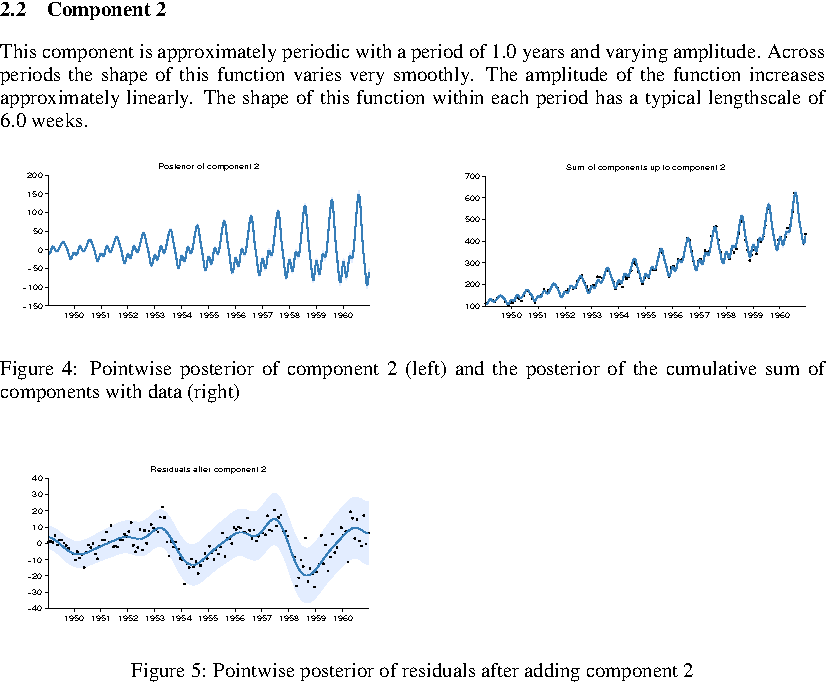
\includegraphics[trim=0.4cm 6cm 8.4cm 2.88cm, clip, width=0.33\columnwidth]{figures/airline-pages/pg_0004-crop} & 
\uptext{$+$} &  
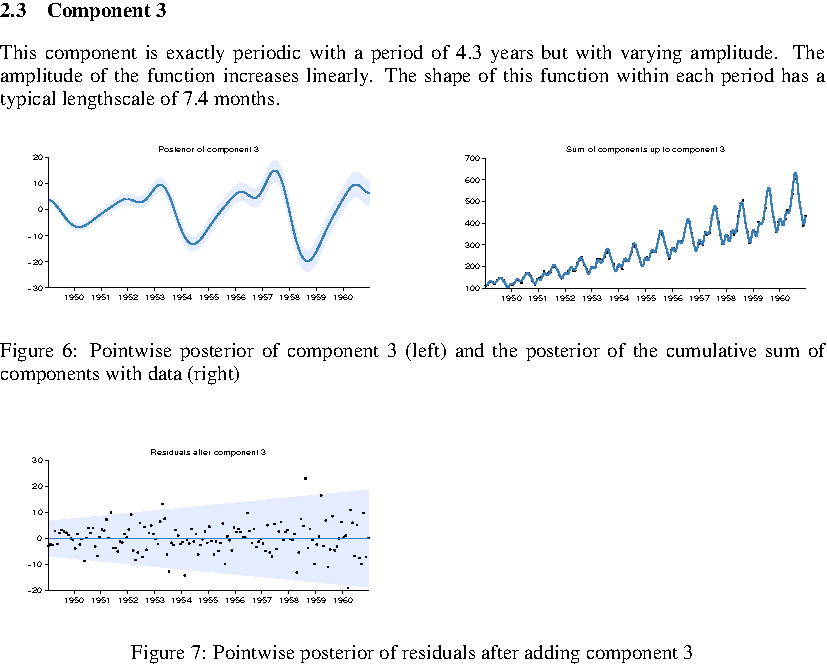
\includegraphics[trim=0.4cm 6cm 8.4cm 2.75cm, clip, width=0.33\columnwidth]{figures/airline-pages/pg_0005-crop} \\
{\scriptsize A very smooth, monotonically increasing function }
& & 
{\scriptsize An approximately periodic function with a period of 1.0 years and with
approximately linearly increasing amplitude}
& & 
{\scriptsize An exactly periodic function with a period of 4.3 years but with linearly
increasing amplitude }
\end{tabular}
\end{tabular}

\end{adjustwidth}
}




\frame[plain]{
\frametitle{A language of regression models}
\begin{itemize} 
	\item We define a language of Gaussian process (GP) regression models by defining a language over kernel functions
	\vspace{\baselineskip}
	\item We start with a small set of base kernels and create a language with a generative grammar
	\begin{itemize}
	  \item Expansion operators include addition, multiplication and change-points
	\end{itemize}
	\vspace{\baselineskip}
	\item The language is open-ended, but its structure makes natural-language description simple
\end{itemize}
}


\frame[plain]{
\frametitle{Kernels determine structure of GPs}
\begin{itemize} 
	\item Kernel determines almost all the properties of a GP prior
	\item Many different kinds, with very different properties:
\end{itemize}
\newcommand{\fhbig}{1.6cm}
\newcommand{\fwbig}{1.8cm}
\newcommand{\kernpic}[1]{\includegraphics[height=\fhbig,width=\fwbig]{figures/structure_examples/#1}}
\newcommand{\kernpicr}[1]{\rotatebox{90}{\includegraphics[height=\fwbig,width=\fhbig]{figures/structure_examples/#1}}}
\newcommand{\addkernpic}[1]{{\includegraphics[height=\fhbig,width=\fwbig]{figures/additive_multi_d/#1}}}
\newcommand{\largeplus}{\tabbox{{\Large+}}}
\newcommand{\largeeq}{\tabbox{{\Large=}}}
\newcommand{\largetimes}{\tabbox{{\Large$\times$}}}
\begin{figure}[ht]
\centering
\renewcommand{\tabularxcolumn}[1]{>{\arraybackslash}m{#1}}
%\begin{tabular}{m{\fwbig}m{0.01\textwidth}m{\fwbig}m{0.01\textwidth}m{\fwbig}m{\fwbig}m{\fwbig}}
%\begin{tabular}{C{\fwbig}C{\fwbig}C{\fwbig}C{\fwbig}}%{m{\fwbig}m{\fwbig}m{\fwbig}}
\begin{tabularx}{\columnwidth}{XXXX}
%Composite & Draws from \gp{} & \gp{} posterior \\ \toprule
  \kernpic{se_kernel} & \kernpic{se_kernel_draws}
& \kernpic{per_kernel} & \kernpic{per_kernel_draws_s2}
\\
  {\small Squared-exp (\kSE)} & {\small local variation} 
& {\small Periodic (\kPer)} & {\small repeating structure}
\\
  \kernpic{lin_kernel} & \kernpic{lin_kernel_draws}
& \kernpic{rq_kernel} & \kernpic{rq_kernel_draws}
\\
  {\small Linear (\kLin)} & {\small linear functions} 
& {\small Rational-quadratic(\kRQ)} & {\small multi-scale variation}
\end{tabularx}
\end{figure}


}


\frame[plain]{
\frametitle{Kernels can be composed}
\begin{itemize} 
	\item Two main operations: addition, multiplication
\end{itemize}
\newcommand{\fhbig}{1.6cm}
\newcommand{\fwbig}{1.8cm}
\newcommand{\kernpic}[1]{\includegraphics[height=\fhbig,width=\fwbig]{figures/structure_examples/#1}}
\newcommand{\kernpicr}[1]{\rotatebox{90}{\includegraphics[height=\fwbig,width=\fhbig]{figures/structure_examples/#1}}}
\newcommand{\addkernpic}[1]{{\includegraphics[height=\fhbig,width=\fwbig]{figures/additive_multi_d/#1}}}
\newcommand{\largeplus}{\tabbox{{\Large+}}}
\newcommand{\largeeq}{\tabbox{{\Large=}}}
\newcommand{\largetimes}{\tabbox{{\Large$\times$}}}
\begin{figure}[ht]
\centering
\renewcommand{\tabularxcolumn}[1]{>{\arraybackslash}m{#1}}
%\begin{tabular}{m{\fwbig}m{0.01\textwidth}m{\fwbig}m{0.01\textwidth}m{\fwbig}m{\fwbig}m{\fwbig}}
%\begin{tabular}{C{\fwbig}C{\fwbig}C{\fwbig}C{\fwbig}}%{m{\fwbig}m{\fwbig}m{\fwbig}}
\begin{tabularx}{\columnwidth}{XXXX}
  \kernpic{lin_times_lin} & \kernpic{lin_times_lin_draws} 
& \kernpic{se_times_per} & \kernpic{se_times_per_draws_s7}
\\
  {\small $\kLin \times \kLin$} & {\small quadratic functions}
& {\small $\kSE \times \kPer$} & {\small locally \newline periodic}
\\
%\midrule 
  \kernpic{lin_plus_per} & \kernpic{lin_plus_per_draws}
& \kernpic{se_plus_per} & \kernpic{se_plus_per_draws_s7}
\\
  {\small $\kLin + \kPer$} & {\small periodic with trend}
& {\small $\kSE + \kPer$ } & {\small periodic with noise}
\end{tabularx}
\end{figure}


}

\frame[plain]{
\frametitle{Kernels can be composed}
\begin{itemize} 
	\item Can be composed across multiple dimensions
\end{itemize}
\newcommand{\fhbig}{1.6cm}
\newcommand{\fwbig}{1.8cm}
\newcommand{\kernpic}[1]{\includegraphics[height=\fhbig,width=\fwbig]{figures/structure_examples/#1}}
\newcommand{\kernpicr}[1]{\rotatebox{90}{\includegraphics[height=\fwbig,width=\fhbig]{figures/structure_examples/#1}}}
\newcommand{\addkernpic}[1]{{\includegraphics[height=\fhbig,width=\fwbig]{figures/additive_multi_d/#1}}}
\newcommand{\largeplus}{\tabbox{{\Large+}}}
\newcommand{\largeeq}{\tabbox{{\Large=}}}
\newcommand{\largetimes}{\tabbox{{\Large$\times$}}}
\begin{figure}[ht]
\centering
\renewcommand{\tabularxcolumn}[1]{>{\arraybackslash}m{#1}}
%\begin{tabular}{m{\fwbig}m{0.01\textwidth}m{\fwbig}m{0.01\textwidth}m{\fwbig}m{\fwbig}m{\fwbig}}
%\begin{tabular}{C{\fwbig}C{\fwbig}C{\fwbig}C{\fwbig}}%{m{\fwbig}m{\fwbig}m{\fwbig}}
\begin{tabularx}{\columnwidth}{XXXX}
  \kernpic{se_times_lin} & \kernpic{se_times_lin_draws_s2}
& \kernpic{lin_times_per} & \kernpic{lin_times_per_draws_s2}
\\
  {\small $\kLin \times \kSE$} & {\small increasing variation}
& {\small $\kLin \times \kPer$} & {\small growing amplitude}
\\
  \addkernpic{additive_kernel} & \addkernpic{additive_kernel_draw_sum}
& \addkernpic{sqexp_kernel}  & \addkernpic{sqexp_draw}
\\
  {\small $\kSE_1 + \kSE_2$} & {\small $f_1(x_1)$ $+ f_2(x_2)$}
& {\small $\kSE_1 \times \kSE_2$} & {\small $f(x_1, x_2)$}
\end{tabularx}
\end{figure}


}



\frame[plain]{
\frametitle{Special cases in our language}
%\begin{center}
%  \begin{tabular}{l|l}
%  Bayesian linear regression & $\Lin$ \\
%  %Bayesian quadratric regression & $\Lin \times \Lin$ \\
%  Bayesian polynomial regression & $\Lin \times \Lin \times \ldots$\\
%  Generalized Fourier decomposition & $\Per + \Per + \ldots$ \\
%  Generalized additive models & $\sum_{d=1}^D \SE_d$ \\
%  Automatic relevance determination & $\prod_{d=1}^D \SE_d$ \\
%  Linear trend with deviations & $\Lin + \SE$ \\
%  Linearly growing amplitude & $\Lin \times \SE$
%  \end{tabular}
%\end{center}
\begin{center}
\begin{tabular}{l|l}
Regression motif & Example kernel \\
\midrule
Linear regression & $\kC + \kLin$ \\
Fourier analysis & $\kC + \sum \cos$ \\
Sparse spectrum \gp{}s & $\sum \cos$ \\
Spectral kernels & $\sum \SE \times \cos$ \\
Changepoints & \eg $\kCP(\kSE, \kSE)$ \\
Kernel smoothing & $\kSE$ \\
Heteroscedasticity & \eg $\kSE + \kLin \times \kWN$ \\
Trend cyclical irregular & $\sum \kSE + \sum \kPer$ \\
Additive nonparametric modelling & $\sum \kSE$ \\
\end{tabular}
\end{center}
}


%\frame[plain]{
%\frametitle{Compositional structure search}
%\begin{itemize}
%	\item Define grammar over kernels:
%	\begin{itemize}
%		\item $ K \rightarrow K + K$ 
%		\item $ K \rightarrow K \times K$ 
%		\item $ K \rightarrow \{ \SE, \Lin, \Per \}$
%	\end{itemize}
%	\vspace{\baselineskip}
%	\item Search the space of kernels greedily by applying local search operators, maximising approximate marginal likelihood.
%\end{itemize}
%}




\tikzset{hide on/.code={\only<#1>{\color{white}}}}

\frame[plain]{
\frametitle{Compositional Structure Search}
\hspace{-1.2cm}
\only<1>{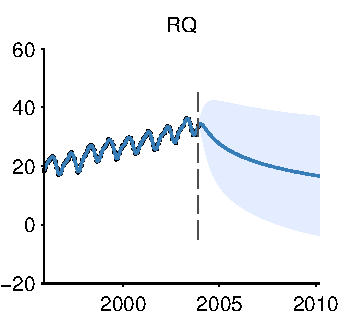
\includegraphics[width=0.4\textwidth]{figures/11-Feb-v4-03-mauna2003-s_max_level_0/03-mauna2003-s_all_small.pdf}}
\only<2>{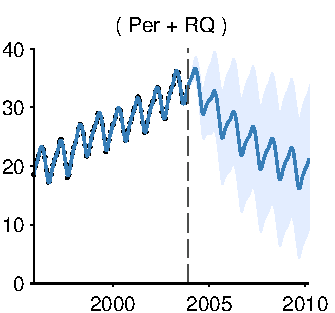
\includegraphics[width=0.4\textwidth]{figures/11-Feb-v4-03-mauna2003-s_max_level_1/03-mauna2003-s_all_small.pdf}}
\only<3>{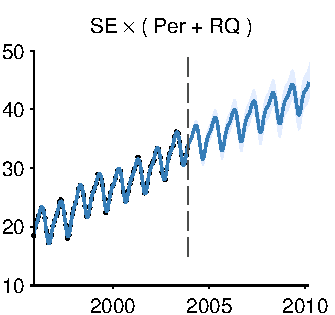
\includegraphics[width=0.4\textwidth]{figures/11-Feb-v4-03-mauna2003-s_max_level_2/03-mauna2003-s_all_small.pdf}}
\only<4>{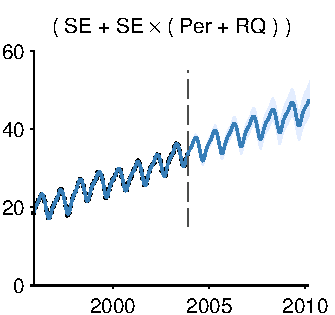
\includegraphics[width=0.4\textwidth]{figures/11-Feb-v4-03-mauna2003-s_max_level_3/03-mauna2003-s_all_small.pdf}}

\vspace{-3.5cm}
\begin{minipage}[t][14cm][t]{1.14\linewidth}
\begin{flushleft}
\hspace{5.5cm}
\vspace{-8cm}
\makebox[\textwidth][c]{
\raisebox{10cm}{
\vspace{-8cm}
\begin{tikzpicture}
[sibling distance=0.18\columnwidth,-,thick, level distance=0.13\columnwidth]
%\footnotesize
\node[shape=rectangle,draw,thick] {Start}
%\pause
  child {node {$\SE$}}
%  fill=camlightblue!30
  child {node[shape=rectangle,draw,thick] {$\RQ$}
    [sibling distance=0.16\columnwidth]
%    {\visible<2->{ child {node {\ldots}}}}
    child [hide on=-1] {node {$\SE$ + \RQ}}
    child [hide on=-1] {node {\ldots}}
    child [hide on=-1] {node[shape=rectangle,draw,thick] {$\Per + \RQ$}
      [sibling distance=0.23\columnwidth]
      child [hide on=-2] {node {$\SE + \Per + \RQ$}}
      child [hide on=-2] {node {\ldots}}
      child [hide on=-2] {node[shape=rectangle,draw,thick] {$\SE \times (\Per + \RQ)$}
        [sibling distance=0.14\columnwidth]
        child [hide on=-3] {node {\ldots}}
        child [hide on=-3] {node {\ldots}}
        child [hide on=-3] {node {\ldots}}
      }
      child [hide on=-2] {node {\ldots}}
    }
    %child {node {$\RQ \times \SE$}}
    child [hide on=-1] {node {\ldots}}
    child [hide on=-1] {node {$\Per \times \RQ$}}
  }
  child {node {$\Lin$}}
  child {node {$\Per$}}
  ;
\end{tikzpicture}}
}\end{flushleft}
\end{minipage}
\only<4>{}
}



\frame[plain]{
\frametitle{Distributivity helps Interpretability}

We can write all kernels as sums of products of base kernels:
$${\SE \times (\RQ + \Lin) = (\SE \times \RQ) + (\SE \times \Lin)}.$$

Sums of kernels are equivalent to sums of functions.

\vspace{\baselineskip}

If $f_1, f_2$ are independent, and ${f_1 \sim \GP(\mu_1, k_1)}$, ${f_2 \sim \GP(\mu_2, k_2)}$ then $${(f_1 + f_2) \sim \GP(\mu_1 + \mu_2, k_1 + k_2)}$$
}

\frame[plain]{
\frametitle{Example Decomposition: Airline }
\begin{center}
  \begin{tikzpicture}[transform canvas={scale=0.9}] 
  \begin{scope}[yshift=0.2\textwidth]
    \begin{scope}[xshift=0cm]
      \node [mybox] (all) at (0, 0) {
        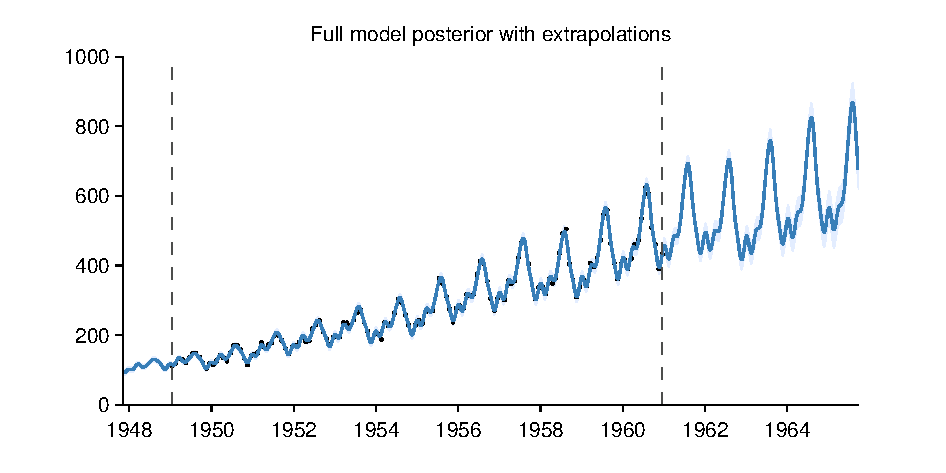
\includegraphics[width=0.8\textwidth, height=0.3\textwidth]{figures/airline/01-airline_all.pdf}
      };
    \end{scope}
  \end{scope}
  \begin{scope}[yshift=0\textwidth]
    \begin{scope}[xshift=0cm]
    \end{scope}
  \end{scope}
  \begin{scope}[yshift=0.27\textwidth]
    \begin{scope}[xshift=5cm]
        \node [mybox, below of=all] (equals) at (0, 0) {\Huge{$=$}};
    \end{scope}
  \end{scope}
  \begin{scope}[yshift=-0.1\textwidth]
    \begin{scope}[xshift=-0.3\textwidth]
      \node [mybox] (all) at (0, 0) {
        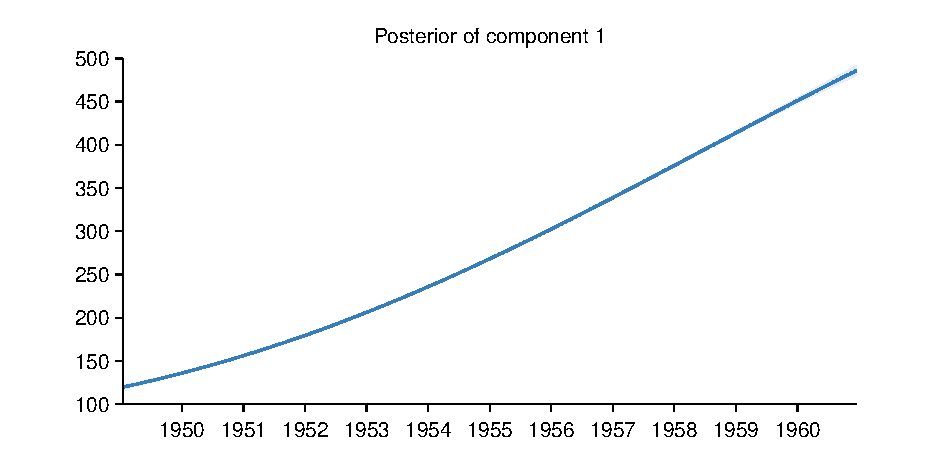
\includegraphics[width=0.5\textwidth]{figures/airline/01-airline_1.pdf}
      };
    \end{scope}
    \begin{scope}[xshift=+0.3\textwidth]
      \node [mybox] (all) at (0, 0) {
        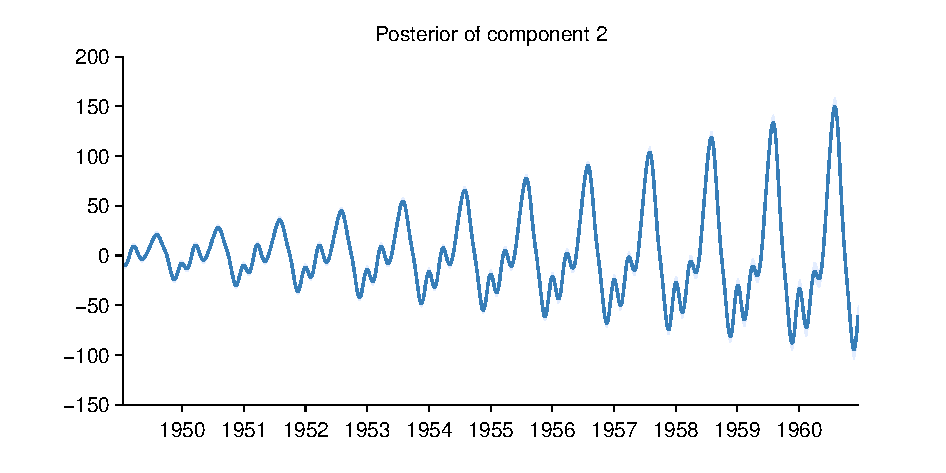
\includegraphics[width=0.5\textwidth]{figures/airline/01-airline_2.pdf}
      };
    \end{scope}
  \end{scope}
  \begin{scope}[yshift=-0.15\textwidth]
    \begin{scope}[xshift=0cm]
        \node [mybox, below of=all] (equals) at (0, 0) {\Huge{+}};
    \end{scope}
  \end{scope}
  \begin{scope}[yshift=-0.35\textwidth]
    \begin{scope}[xshift=-0.3\textwidth]
      \node [mybox] (all) at (0, 0) {
        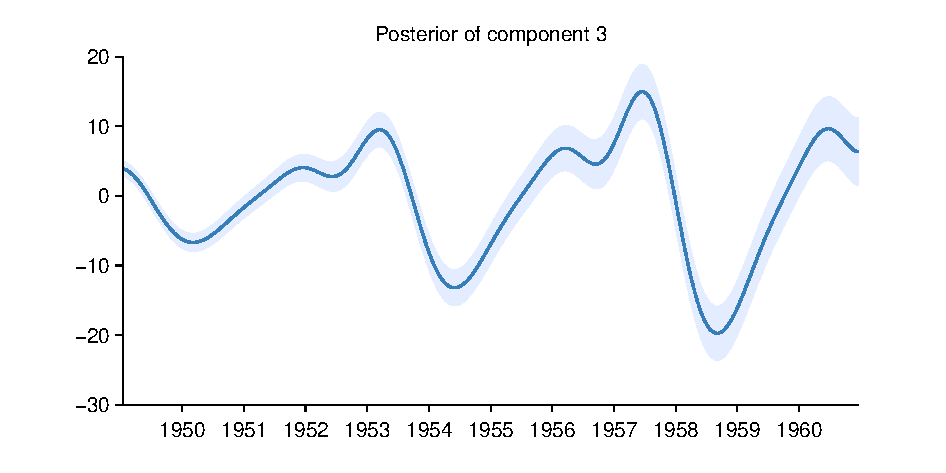
\includegraphics[width=0.5\textwidth]{figures/airline/01-airline_3.pdf}
      };
    \end{scope}
    \begin{scope}[xshift=+0.3\textwidth]
      \node [mybox] (all) at (0, 0) {
        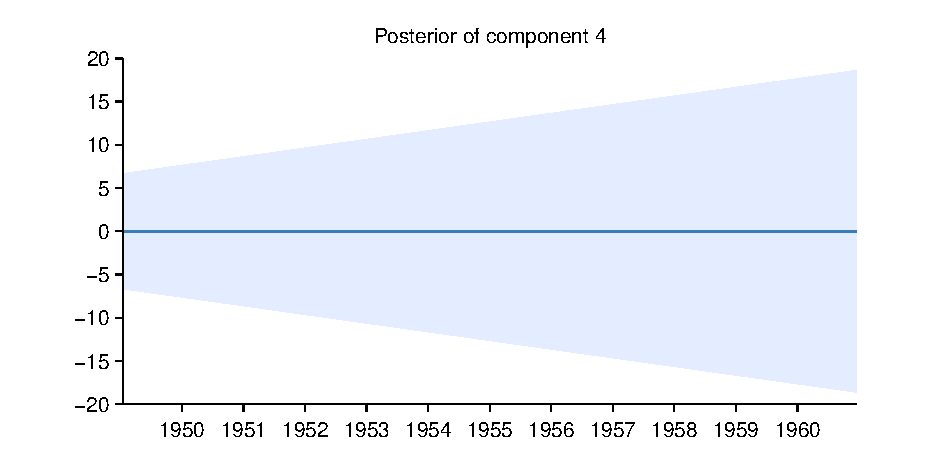
\includegraphics[width=0.5\textwidth]{figures/airline/01-airline_4.pdf}
      };
    \end{scope}
  \end{scope}
\end{tikzpicture}

\end{center}
}


\frame[plain]{
\frametitle{Example Kernel Descriptions}
\centering
\begin{tabular}{l|l}
Product of Kernels & Description \\
\midrule
$\kPer$ & An exactly periodic function \\
$\kPer \times \kSE$ & An approximately periodic function \\
$\kPer \times \kSE \times \kLin$ & An approximately periodic function \\ &  with linearly varying amplitude \\
$\kLin$ & A linear function \\
$\kLin \times \kLin$ & A quadratic function \\
$\kPer \times \kLin \times \kLin$ & An exactly periodic function \\ & with quadratically varying amplitude\\
\end{tabular}
}


\frame[plain]{
\frametitle{This analysis was automatically generated}

\vspace{0.5\baselineskip}

\begin{center}
\fbox{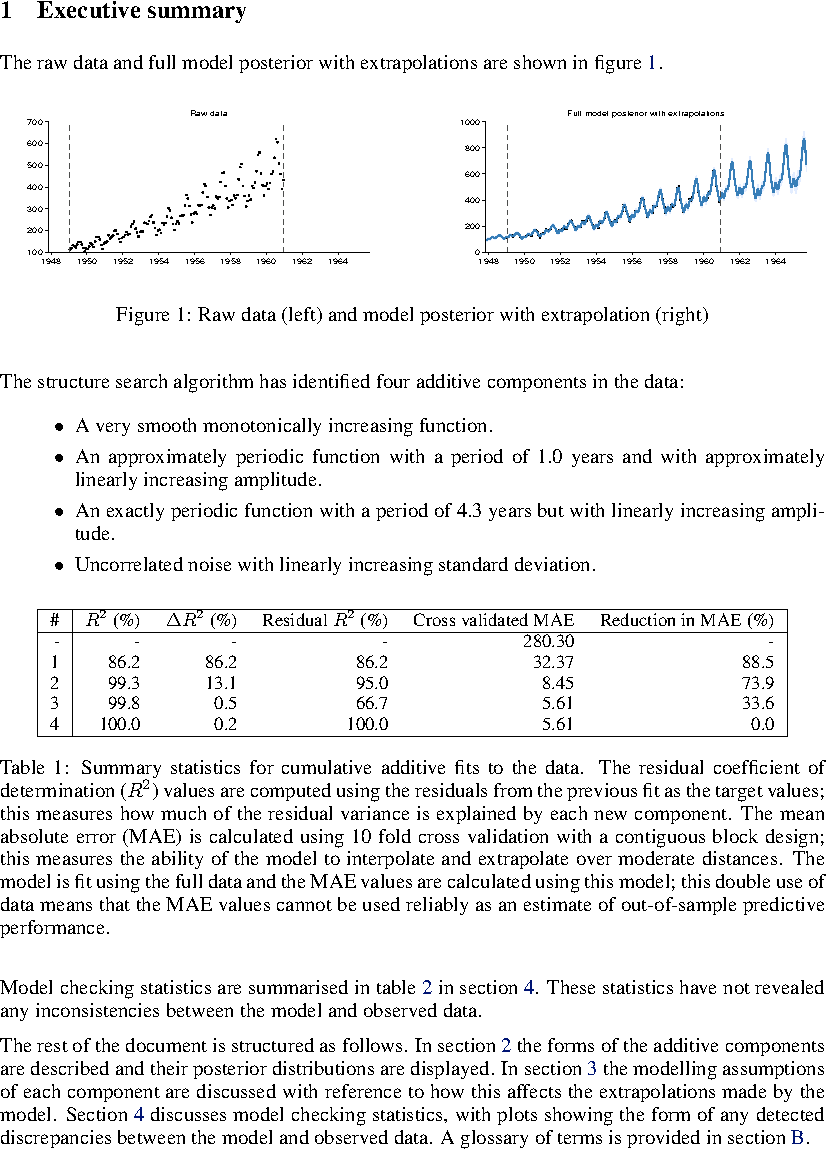
\includegraphics[trim=0cm 9.5cm 0cm 0.7cm, clip, width=0.98\columnwidth]{figures/airline-pages/pg_0002-crop.pdf}}


\end{center}
}

\frame[plain]{
\frametitle{This analysis was automatically generated}

\begin{center}
\vspace{0.5\baselineskip}

\only<1>{
\fbox{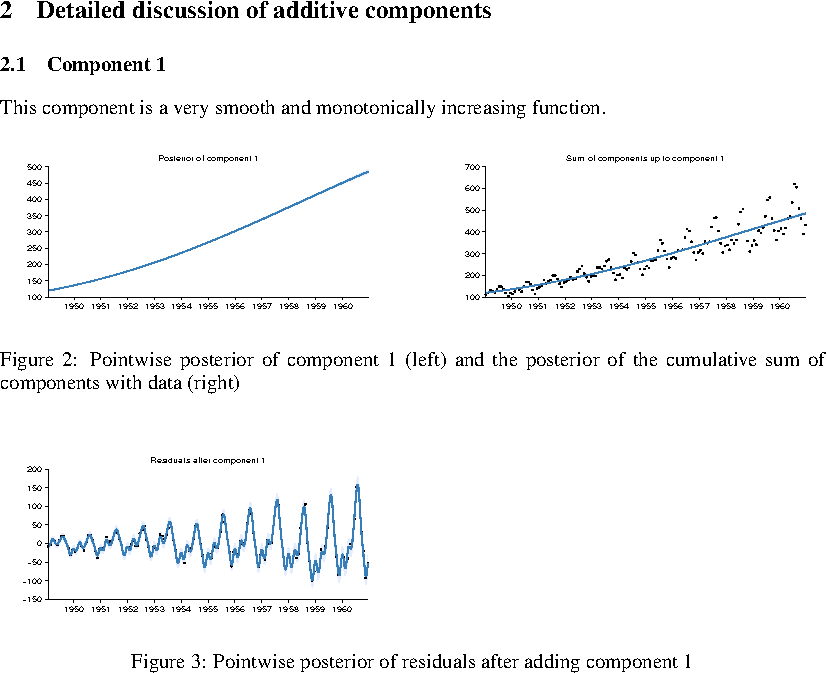
\includegraphics[trim=0cm 6cm 0cm 0.9cm, clip, width=0.98\columnwidth]{figures/airline-pages/pg_0003-crop.pdf}}}

\only<2>{\fbox{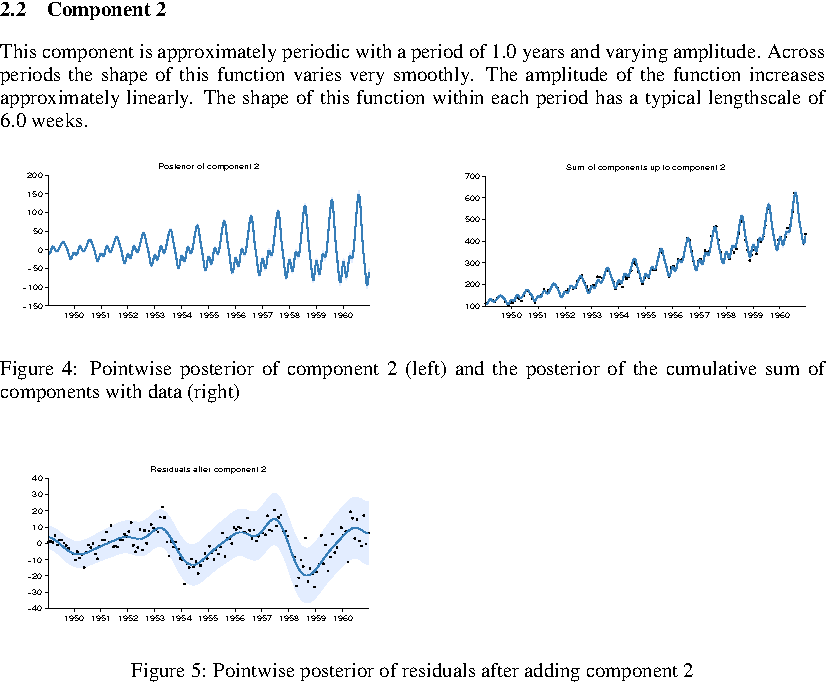
\includegraphics[trim=0cm 6cm 0cm 0.0cm, clip, width=0.98\columnwidth]{figures/airline-pages/pg_0004-crop.pdf}}}

\only<3>{
\fbox{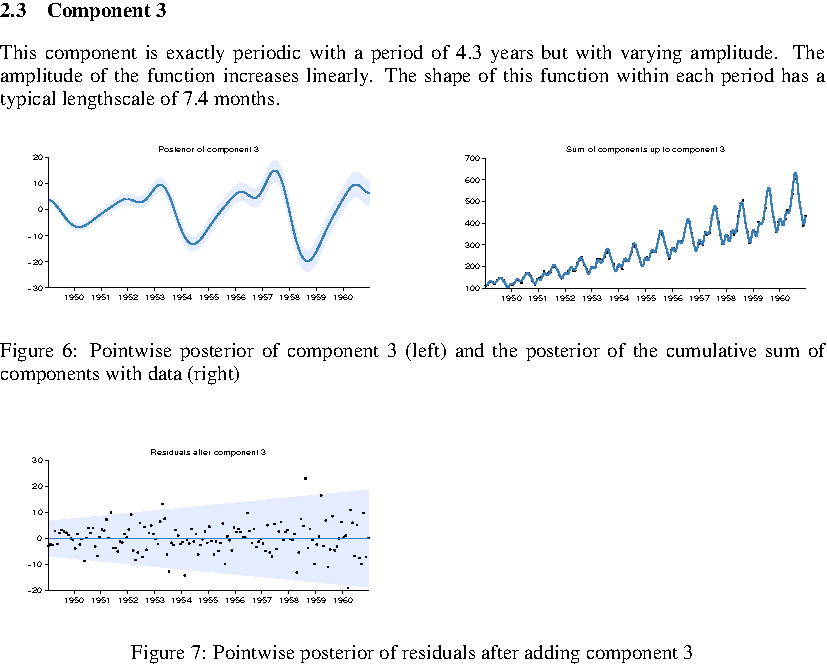
\includegraphics[trim=0cm 6cm 0cm 0.0cm, clip, width=0.98\columnwidth]{figures/airline-pages/pg_0005-crop.pdf}}}

\end{center}
}






\frame[plain]{
\frametitle{Summary}
\begin{itemize}
	\item Constructed a language of regression models via kernel composition
	\vspace{\baselineskip}
	\item Searched over this language greedily
	\vspace{\baselineskip}
	\item Kernels modify prior in predictable ways, allowing automatic natural-language description of models
	\vspace{\baselineskip}
\end{itemize}
	\pause
	\centering
	{
		\hfill
		Thanks!
				\hfill
	}
}



\end{document}